\subsection{Rancangan Detail Komponen}
\label{subsection:detail-komponen}

Berdasarkan rancangan struktural yang sudah dijelaskan pada bagian \ref{subsection:rancangan-struktural}, sistem akan diimplementasikan sebagai kumpulan komponen. Masing-masing komponen tersebut memiliki peran dan tanggung jawab yang berbeda dalam sistem eksperimen.

\subsubsection{Rancangan Detail Node}
\label{subsubsection:detail-node}

Seperti yang sudah dijelaskan pada Bagian \ref{subsubsection:node}, \textit{Node} merupakan satuan fungsional utama yang berperan sebagai entitas dalam sistem \textit{database} terdistribusi yang dikembangkan. Selain komponen yang telah disebutkan pada bagian tersebut, \textit{Node} juga memiliki komponen internal yang berfungsi untuk menghasilkan data \textit{trace} yang dapat digunakan untuk keperluan \textit{debugging} dan analisis kinerja sistem serta konfigurasi yang mengatur perilaku \textit{Node}. Ilustrasi struktur \textit{Node} yang lebih detail dapat dilihat pada Gambar \ref{fig:node-structure}.

Komponen internal lain dalam \textit{Node} adalah jalur komunikasi \textit{message passing} antara antarmuka \textit{client}, antarmuka antar-\textit{Node}, dan komponen konsensus. Hal ini disebabkan karena modularitas implementasi OmniPaxos yang tidak mengintegrasikan komponen konsensus dengan antarmuka jaringan.

Implementasi \textit{erasure coding} bukan terdapat pada \textit{Node} melainkan pada komponen OmniPaxos. Alasan untuk hal ini adalah kompleksitas perubahan dari konsensus yang perlu dilakukan ketika operasi diubah menjadi menggunakan \textit{erasure coding}. Dengan demikian, komponen OmniPaxos akan menangani operasi \textit{erasure coding} dan replikasi data, sementara \textit{Node} akan menerima hasil dari OmniPaxos untuk melanjutkan operasi ke penyimpanan data dan komunikasi antar-\textit{Node}. Detail implementasi \textit{erasure coding} akan dibahas pada Bagian \ref{subsubsection:detail-komponen-konsensus}.

\begin{figure}[ht]
    \centering
    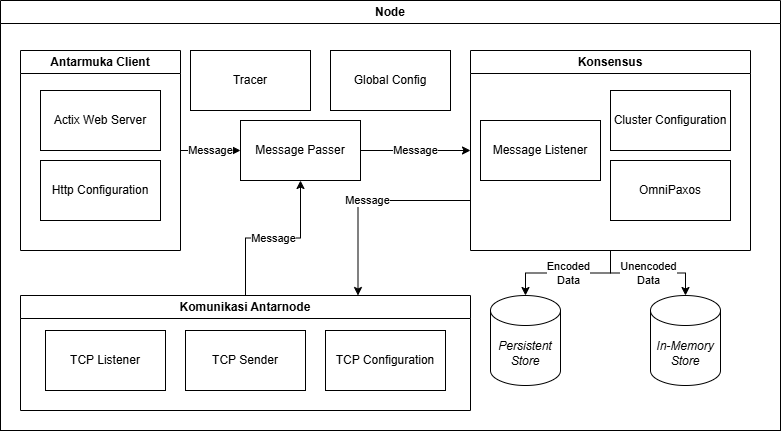
\includegraphics[width=0.95\textwidth]{resources/chapter-3/node-architecture.png}
    \caption{Struktur Node}
    \label{fig:node-structure}
\end{figure}

\subsubsection{Rancangan Detail Komponen Konsensus}
\label{subsubsection:detail-komponen-konsensus}

Komponen konsensus bertanggung jawab untuk menjaga konsistensi data antar-\textit{Node} dalam sistem. Komponen ini akan mengimplementasikan algoritma konsensus yang diperlukan untuk mencapai kesepakatan di antara \textit{Node} dalam hal status dan nilai data seperti yang sudah dijelaskan di Bagian \ref{subsection:konsensus}.

Algoritma yang digunakan dalam komponen konsensus sesuai pertimbangan di Bagian \ref{subsubsection:pemilihan-algoritma-konsensus} adalah OmniPaxos. Algoritma ini diadaptasi untuk memenuhi kebutuhan spesifik dari sistem yang sedang dibangun, yaitu dengan menambahkan dukungan untuk \textit{erasure coding} dalam proses konsensus. OmniPaxos sudah memiliki desain yang modular sehingga memudahkan penyesuaian terhadap kebutuhan sistem. Ilustrasi struktur komponen konsensus dapat dilihat pada Gambar \ref{fig:consensus-component-structure}.

Kondisi yang disimpan oleh komponen konsensus terdapat pada bagian \textit{Sequence Paxos} yang berfungsi untuk menyimpan \textit{state} dari \textit{Node}, termasuk status \textit{leader}, \textit{follower}, \textit{log number}, dan informasi lainnya yang diperlukan untuk mencapai konsensus. Selain itu, OmniPaxos juga terhubung ke dalam sebuah penyimpanan data yang digunakan untuk menyimpan \textit{log} dari transaksi. Penyimpanan ini berbeda dengan \textit{Key-value store} yang digunakan oleh \textit{Node} untuk menyimpan data yang direplikasi atau di-\textit{erasure code}. Penyimpanan ini akan digunakan untuk menyimpan \textit{log} dari transaksi dan bersifat lokal, namun akan digunakan sebagai \textit{fallback} jika terjadi kegagalan pada \textit{Node}.

Selain itu, komponen OmniPaxos bertanggung jawab untuk melakukan operasi \textit{erasure coding} pada data jika sistem menggunakan skema tersebut. Skema \textit{erasure coding} menyebabkan data yang ditransaksikan menjadi tidak sama antara \textit{Node} yang satu dengan yang lainnya. Penggunaan \textit{erasure coding} juga mengubah jumlah \textit{Node} yang diperlukan untuk mencapai kuorum, mengikuti referensi pada Bagian \ref{subsection:paxos-erasure}. Dengan demikian, lebih mudah jika komponen \textit{erasure coding} berada pada komponen utama yang berkaitan dengan konsensus. Komponen \textit{erasure coding service} akan menyimpan konfigurasi \textit{data shard} dan \textit{parity shard} yang digunakan untuk melakukan operasi \textit{erasure coding}. Komponen ini juga melakukan operasi \textit{erasure coding} pada data yang diterima dari \textit{Node} dan mengembalikan hasilnya ke \textit{Node}.

\begin{figure}[ht]
    \centering
    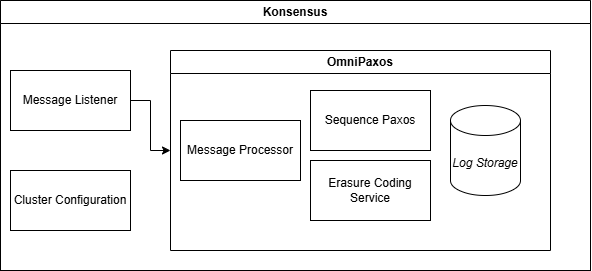
\includegraphics[width=0.85\textwidth]{resources/chapter-3/consensus-architecture.png}
    \caption{Struktur Komponen Konsensus}
    \label{fig:consensus-component-structure}
\end{figure}

\subsubsection{Rancangan Detail Antarmuka Client}
\label{subsubsection:detail-client-interface}

Antarmuka \textit{client} bertanggung jawab untuk menyediakan akses ke sistem bagi pengguna. Antarmuka ini akan menyediakan fungsi yang dibutuhkan, yaitu \textit{read} dan \textit{write} data. Antarmuka ini juga dapat digunakan pengguna untuk melihat status sistem, seperti status \textit{Node}, status \textit{Cluster}, dokumentasi, dan informasi lainnya yang diperlukan. Antarmuka \textit{client} akan dibuat memanfaatkan protokol HTTP. Alasan dari pemilihan protokol HTTP adalah karena protokol ini sudah umum digunakan dan didukung oleh banyak bahasa pemrograman maupun alat. Selain itu, protokol HTTP juga mudah digunakan dan dapat diakses melalui berbagai platform, termasuk web browser. Dukungan alat terhadap protokol HTTP akan memudahkan pengembangan dan pengujian sistem. Rancangan antarmuka \textit{client} dapat dilihat pada gambar \ref{fig:client-interface-component}.

\begin{figure}[ht]
    \centering
    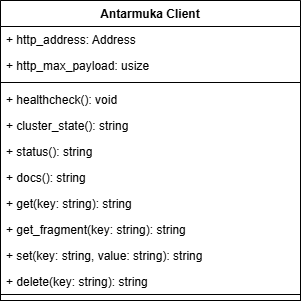
\includegraphics[width=0.45\textwidth]{resources/chapter-3/client-interface-component.png}
    \caption{Komponen Antarmuka Client}
    \label{fig:client-interface-component}
\end{figure}

Antarmuka tersebut akan terhubung pada \textit{endpoint} HTTP yang disediakan. Fungsi yang ada akan dieksekusi ketika \textit{request} diterima pada \textit{endpoint} yang sesuai.
\subsubsection{Rancangan Detail Komunikasi Antarnode}
\label{subsubsection:detail-komponen-internode-interface}

Komponen komunikasi antarnode bertanggung jawab untuk mengelola komunikasi antar node dalam sistem. Komponen ini berperan sebagai antarmuka yang digunakan komponen konsensus untuk berkomunikasi dengan node lain. Antarmuka akan berjalan menggunakan protokol TCP dengan abstraksi aplikasi dibuat secara manual. Hal ini dilakukan untuk meningkatkan kinerja dari sistem. Rancangan antarmuka komunikasi antarnode dapat dilihat pada Gambar \ref{fig:internode-interface-component}.

\begin{figure}[ht]
	\centering
	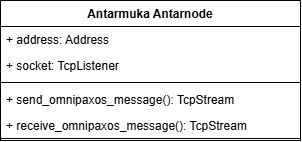
\includegraphics[width=0.45\textwidth]{resources/chapter-3/internode-interface-component.png}
	\caption{Komponen Antarmuka Komunikasi Antarnode}
	\label{fig:internode-interface-component}
\end{figure}

Antarmuka tersebut hanya menyediakan fungsi untuk mengirim dan menerima pesan. Abstraksi aplikasi yang perlu dilakukan adalah melakukan \textit{encode} pesan ke bentuk yang dapat dikenali oleh sistem dan \textit{multiplexing} agar pesan dari banyak sumber dapat diproses sesuai kebutuhan tanpa konflik dengan pesan lainnya mengingat pesan disimpan pada \textit{socket} yang sama menggunakan mekanisme \textit{queue}.
\subsubsection{Rancangan Detail Persistent Store}
\label{subsubsection:detail-persistent-store}

Komponen \textit{Persistent Store} bertanggung jawab untuk menyimpan data secara permanen. Komponen ini akan menggunakan sistem penyimpanan yang sesuai untuk memastikan bahwa data dapat disimpan dan diambil. Sesuai dengan bagian \ref{subsubsection:persistent-database}, komponen ini menggunakan RocksDB sebagai basis data penyimpanan. Rancangan komponen dapat dilihat pada gambar \ref{fig:persistent-store-component}.

\begin{figure}[ht]
    \centering
    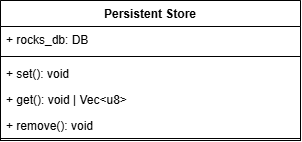
\includegraphics[width=0.4\textwidth]{resources/chapter-3/persistent-store-component.png}
    \caption{Komponen Persistent Store}
    \label{fig:persistent-store-component}
\end{figure}
\subsubsection{Rancangan Detail In-Memory Store}
\label{subsubsection:detail-in-memory-store}

Komponen \textit{In-Memory Store} bertanggung jawab untuk menyimpan data secara sementara dalam memori. Komponen ini akan menggunakan struktur data yang sesuai untuk memastikan bahwa data dapat disimpan dan diambil dengan cepat. Sesuai dengan Bagian \ref{subsubsection:in-memory-kv-store}, komponen ini menggunakan Moka sebagai sistem \textit{cache}. Rancangan komponen dapat dilihat pada Gambar \ref{fig:in-memory-store-component}.

\begin{figure}[ht]
    \centering
    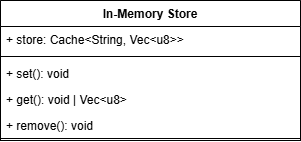
\includegraphics[width=0.4\textwidth]{resources/chapter-3/in-memory-store-component.png}
    \caption{Struktur Komponen In-Memory Store}
    \label{fig:in-memory-store-component}
\end{figure}
\subsubsection{Rancangan Detail Data Collector}
\label{subsubsection:detail-data-collector}

Seperti yang sudah dijelaskan pada bagian \ref{subsubsection:data-collector}, \textit{Data Collector} merupakan komponen yang bertanggung jawab untuk mengumpulkan data eksperimen dari sistem yang sedang diuji. Komponen ini berperan penting dalam menyediakan data yang diperlukan untuk analisis kinerja dan evaluasi sistem. Selain itu, \textit{Data Collector} juga menyediakan antarmuka yang memungkinkan pengguna untuk melakukan eksperimen dengan sistem menggunakan variabel jumlah \textit{virtual user}, ukuran data, \textit{bandwidth}, dan konfigurasi sistem yang digunakan. Ilustrasi struktur \textit{Data Collector} yang lebih detail dapat dilihat pada gambar \ref{fig:data-collector-structure}.

\begin{figure}[ht]
    \centering
    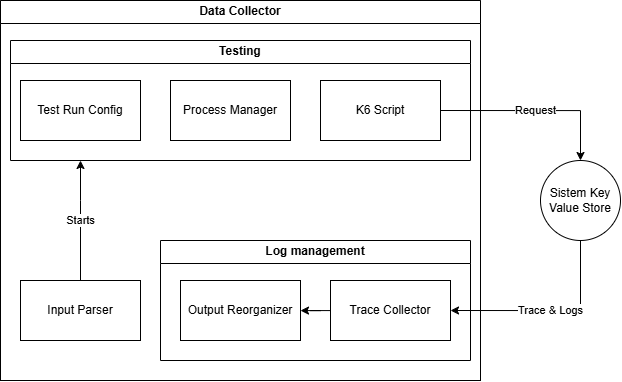
\includegraphics[width=0.75\textwidth]{resources/chapter-3/data-collector-architecture.png}
    \caption{Struktur Data Collector}
    \label{fig:data-collector-structure}
\end{figure}

Komponen internal yang ada pada \textit{Data Collector} adalah \textit{Input Parser} yang berfungsi untuk mem-parsing input dari pengguna dan \textit{Config Parser} yang berfungsi untuk membaca konfigurasi sistem yang digunakan dalam eksperimen untuk kemudian dibangun.
\subsubsection{Rancangan Detail Komponen Benchmark}
\label{subsubsection:detail-data-benchmark}

Komponen \textit{benchmark} bertanggung jawab untuk melakukan pengujian terhadap sistem yang telah dibangun. Pengujian ini juga bertujuan menghasilkan data analisis. Komponen \textit{benchmark} dapat mengatur variabel melalui \textit{Test Run Config}. Variabel ini kemudian digunakan untuk membuat \textit{Test Execution Loop} yang akan mengeksekusi semua kombinasi dari variabel yang telah ditentukan. Dalam setiap iterasi dari \textit{Test Execution Loop} akan membangun sistem menggunakan \textit{Process Manager}. \textit{Process Manager} akan mengelola proses sistem yang akan diuji dengan masing-masing \textit{Node} berada pada proses yang berbeda. Setelah sistem dibangun, \textit{Process Manager} akan mengirimkan perintah untuk memulai sistem dan menyimpan \textit{PID} dari setiap proses yang berjalan. Pengujian akan dilakukan dengan k6 yang akan mengirimkan \textit{request} ke sistem yang sedang diuji. Ilustrasi struktur komponen \textit{benchmark} dapat dilihat pada gambar \ref{fig:benchmark-structure}.

\begin{figure}[ht]
    \centering
    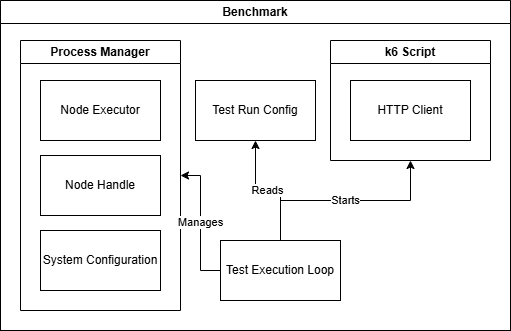
\includegraphics[width=0.55\textwidth]{resources/chapter-3/benchmark-architecture.png}
    \caption{Struktur Komponen Benchmark}
    \label{fig:benchmark-structure}
\end{figure}

Setelah pengujian selesai, \textit{Process Manager} akan mengirimkan perintah untuk menghancurkan sistem yang diuji dan membuat ulang dengan konfigurasi selanjutnya. Pengujian akan diulang hingga semua kombinasi dari variabel yang telah ditentukan selesai dieksekusi.
\subsubsection{Rancangan Detail Komponen Log Management}
\label{subsubsection:detail-data-log-management}

Komponen \textit{logging} dan \textit{tracing} bertanggung jawab untuk mencatat dan melacak aktivitas sistem. Komponen ini akan mengumpulkan data dari berbagai komponen lain dalam sistem, termasuk informasi tentang permintaan yang diterima, respons yang dikirim, dan status sistem secara keseluruhan. Ilustrasi struktur komponen \textit{log management} dapat dilihat pada gambar \ref{fig:log-management-structure}.

\begin{figure}[ht]
    \centering
    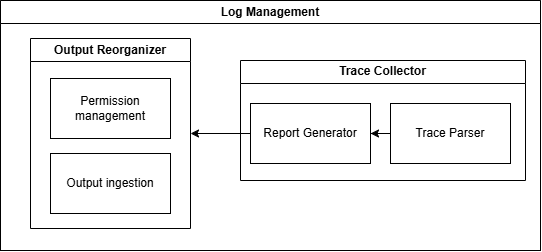
\includegraphics[width=0.55\textwidth]{resources/chapter-3/log-management-architecture.png}
    \caption{Struktur Komponen Log Management}
    \label{fig:log-management-structure}
\end{figure}

Tugas komponen \textit{log management} relatif sederhana, yaitu mengumpulkan data dari hasil \textit{log} yang dihasilkan \textit{node} lalu membangun laporan dari data tersebut yang dapat dikelola. Selain itu, komponen ini juga mengotomasi organisasi data yang dihasilkan dari \textit{benchmark}. Data ini kemudian akan digunakan untuk analisis lebih lanjut.
